% wsq 这应该算是motivation实验,基于这个观察你才有空间去选择策略。不应该出现在大实验中。
\section{研究意义}

本文选用OPT-13B、OPT-30B、Llama-13B和Llama-32.5B进行实验,针对单个用户请求,测试张量交换与张量重算开销随序列长度的变化关系。其结果如图\ref{Fig:交换与重算开销对比}所示。当序列长度较小时,交换开销小于重算开销。随着序列长度的增加,二者大小关系反转。

\begin{figure}[!htbp]
    \centering
    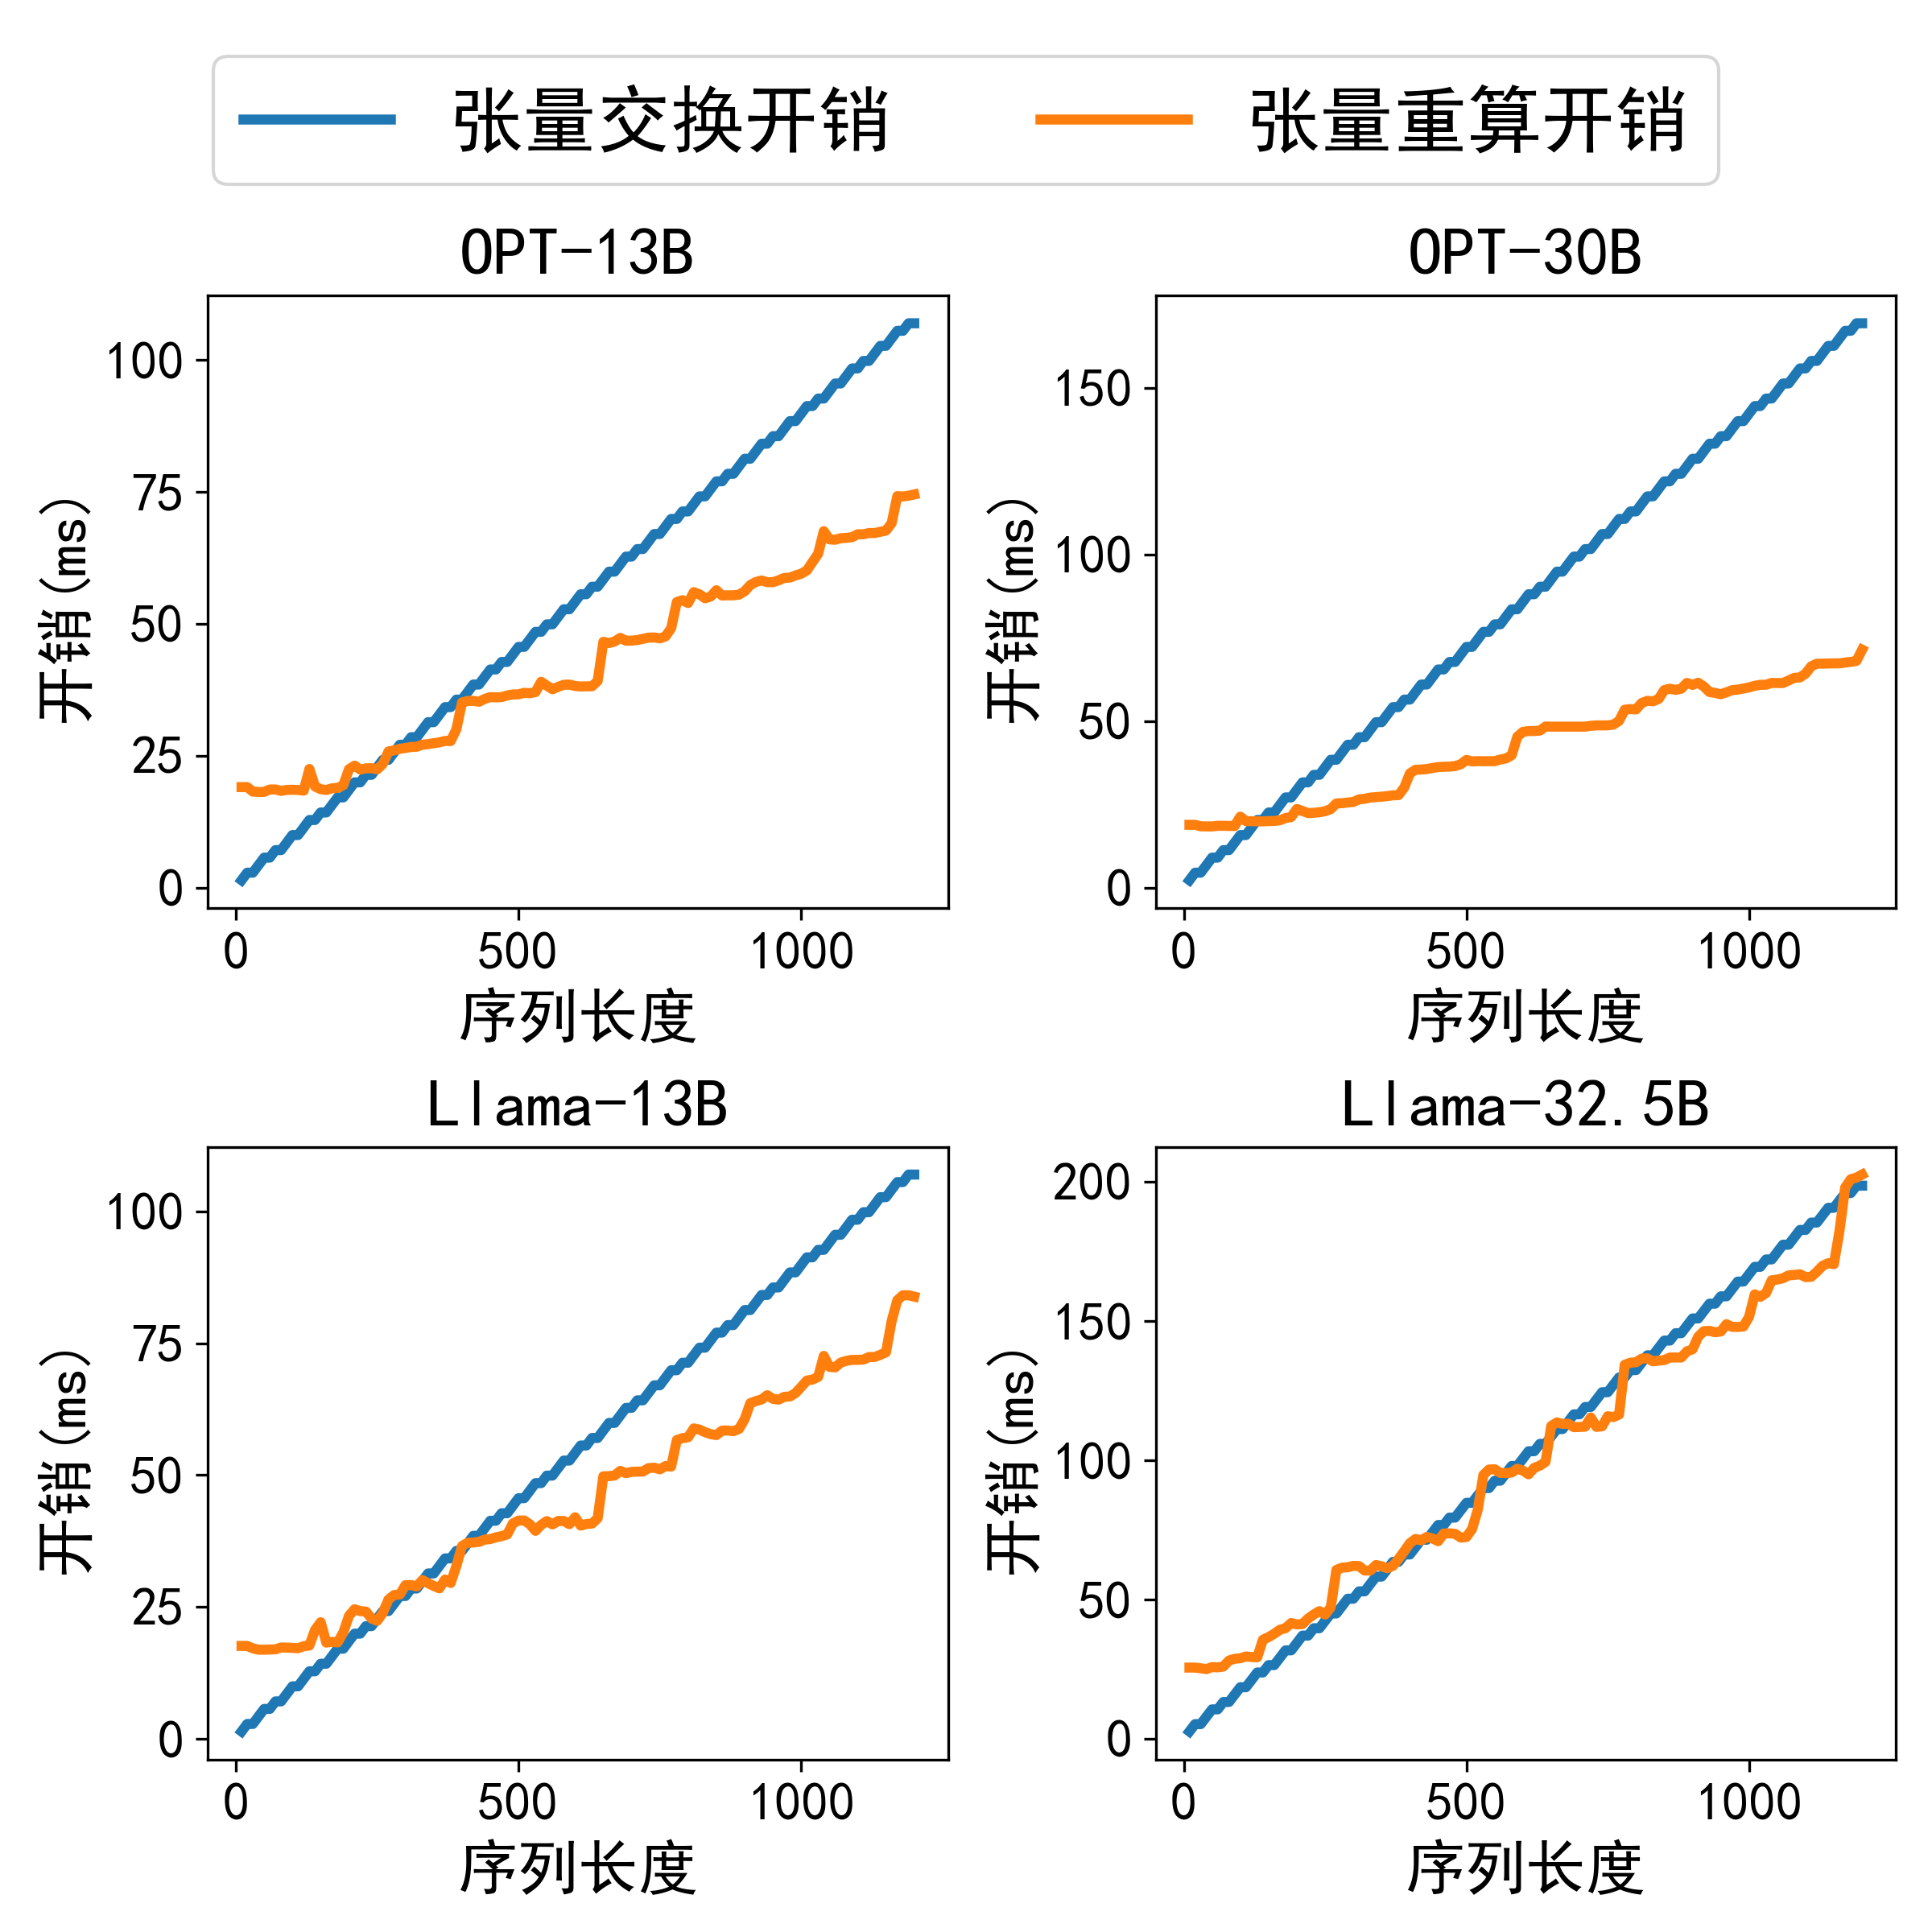
\includegraphics[width=0.85\linewidth]{交换与重算开销对比.png}
    \caption{交换与重算开销对比}
    \label{Fig:交换与重算开销对比}
  \end{figure}

\begin{itemize}    
    \item \textbf{张量重算开销}:自注意力机制内核采用并行计算策略,每个线程只计算一个token的qkv张量及注意力值。随着序列长度的增长,线程数量增加,同步开销随之上升,而单线程计算量不变,导致张量重算开销随序列长度增加呈亚线性增长。
    \item \textbf{张量交换开销}:KV Cache保存每个token的key-value张量,其内存占用与序列长度呈正比关系,而PCIe传输带宽在推理过程中基本保持稳定。因此张量交换开销与序列长度也呈正比关系。
\end{itemize}

因此,张量重算开销随序列长度的增长速度小于张量交换开销。在贪心采样策略下,对于长序列而言,无论是vLLM还是AdaptiveLLM,都使用张量重算,两种策略带来内存优化行为没有差异。对于短序列而言,vLLM使用张量重算,而AdaptiveLLM使用开销较小的张量交换,此时能够带来整体吞吐率提升。且OPT-13B和Llama-13B相比于OPT-30B和Llama-32.5B,在序列长度较短时,张量交换相比于张量重算,开销优势更加明显。

在LLM实际应用场景中,大多数序列的长度较短,使得张量交换在提升性能上拥有明显优势。而当长序列较多,或者CPU内存空间不足时,张量重算技术能够发挥优势。AdaptiveLLM能够基于服务器软硬件环境、LLM与数据集选取、用户参数设置与推理任务运行时信息来精准预测张量交换与张量重算开销,并选择开销较小的内存优化技术执行。 
